The large area APDs enabled the Ecal to have the sensitivity to detect signals from cosmic muons traversing the Ecal crystals perpendicularly and then to use this signal for the initial calibration of the modules. The experimental setup was modeled using Monte Carlo simulations so that the energy deposited in the crystals from cosmic ray muons and rates could be studied. By measuring the average path length of cosmic ray muons in each crystal, the energy deposited in each crystal of the Ecal was calculated using the known energy deposition from 2~GeV muons \cite{Olive}. 

The experimental setup for the cosmic calibrations utilized two scintillators placed below the Ecal to trigger readout of all of the crystals. A schematic for the setup of the cosmic calibration is shown in Fig.~\ref{Figure:cosmicScheme}.

%include some discussion of the improvement achieved after removing the splitters

\begin{figure}[H]
  \centering
      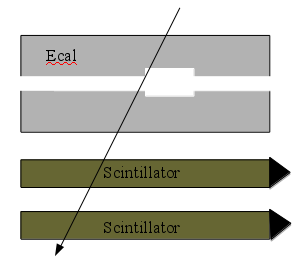
\includegraphics[width=0.5\textwidth]{pics/performance/cosmicschematic.png}
  \caption[Setup for Ecal cosmic ray calibration]{Experimental setup for the cosmic ray calibration. As a cosmic ray passe vertically through both scintillators, event readout is triggered.}
  \label{Figure:cosmicScheme}
\end{figure}

Each scintillator measures 75~cm long, 22~cm wide and 5~cm thick covering a slightly larger perpendicular area than the Ecal crystals. The two scintillators are less than half a meter apart with the closest scintillator less than half a meter beneath the Ecal. The energy deposited in each crystal in a layer is sensitive to the path length of the track as it passed through the crystal. Simulations show the average energy deposited in a crystal by a triggering vertical track in the scintillators in Fig.~\ref{Figure:cosmicEdep}.

\begin{figure}[H]
  \centering
      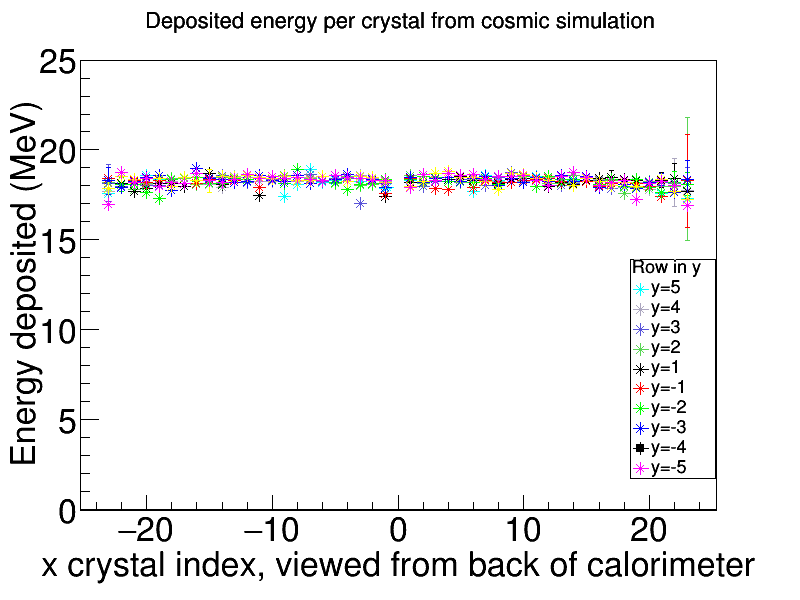
\includegraphics[width=0.8\textwidth]{pics/performance/cosmicEdep.png}
  \caption[Simulation of energy deposited per Ecal module from cosmic rays]{The simulated cosmic ray muon energy deposition per crystal of the Ecal. The mean energy was 18.3~MeV.}
  \label{Figure:cosmicEdep}
\end{figure}

In Fig.~\ref{Figure:cosmicEdep}, only tracks passing through one crystal in a row were included. Additinally, the cosmic ray muon track had to pass through an adjacent crystal in the rows above and below a crystal. For crystals near edges, the geometrical requirement was adjusted to include the two crystals immediately above (or below for cases where the edge is above the crystal) the crystal being readout. The average energy deposited per crystal is approximately 18.3~MeV in agreement with the PDG. 

In data, the raw FADC waveform for each crystal is readout, and the event is kept for further study after applying strict coincidence cuts between the two scintillators. The trigger rate for data is about 7~Hz. Only 30$\%$ of events passed the coincidence cut between the scintillators. For a track passing vertically through all ten layers, we can see the signal in each crystal as shown in Fig.~\ref{Figure:cosmicSig}.

\begin{figure}[H]
  \centering
      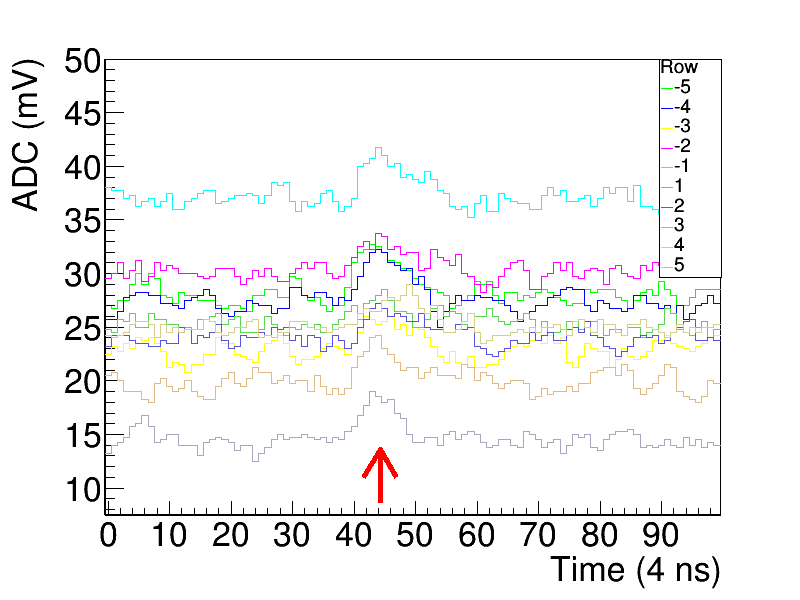
\includegraphics[width=0.7\textwidth]{pics/performance/cosmicSignal.png}
  \caption[Real cosmic ray signal in raw FADC waveform passing vertically through Ecal]{Cosmic ray signal passing vertically through all ten layers of crystals in the Ecal. Each crystal's signal is separated vertically in this plot by an offset (pedestal). The arrow indicates the approximate place in time that the cosmic signal passed through the detector.}
  \label{Figure:cosmicSig}
\end{figure}

As seen in Fig.~\ref{Figure:cosmicSig}, each FADC channel has a unique pedestal value. The pedestal for each event was calculated as an average of the first twenty bins of the time window. The integrated signal was used for the final calibration. By searching for a threshold crossing in the time window where cosmic events occurred, the signal was then fully integrated and the pedestal was subtracted. The raw waveform thresholds were 2.5~mV in 2015 and increased to 3.5~mV in 2016 to accommodate the larger signals after the removal of the splitters. Geometric cuts are then applied to the data in offline analysis. Crystals having peaks over a certain threshold must have at least an adjacent crystals located above and below with threshold crossing, but the crystals to the left and right must not cross threshold. These cuts ensure that that the track passed as vertically as possible through the Ecal (reducing the variations in path length across each crystal). The integrated signals over many events in each crystal were fit. An individual crystal fit is shown in Fig.~\ref{Figure:cosmicFit}.

\begin{figure}[H]
  \centering
      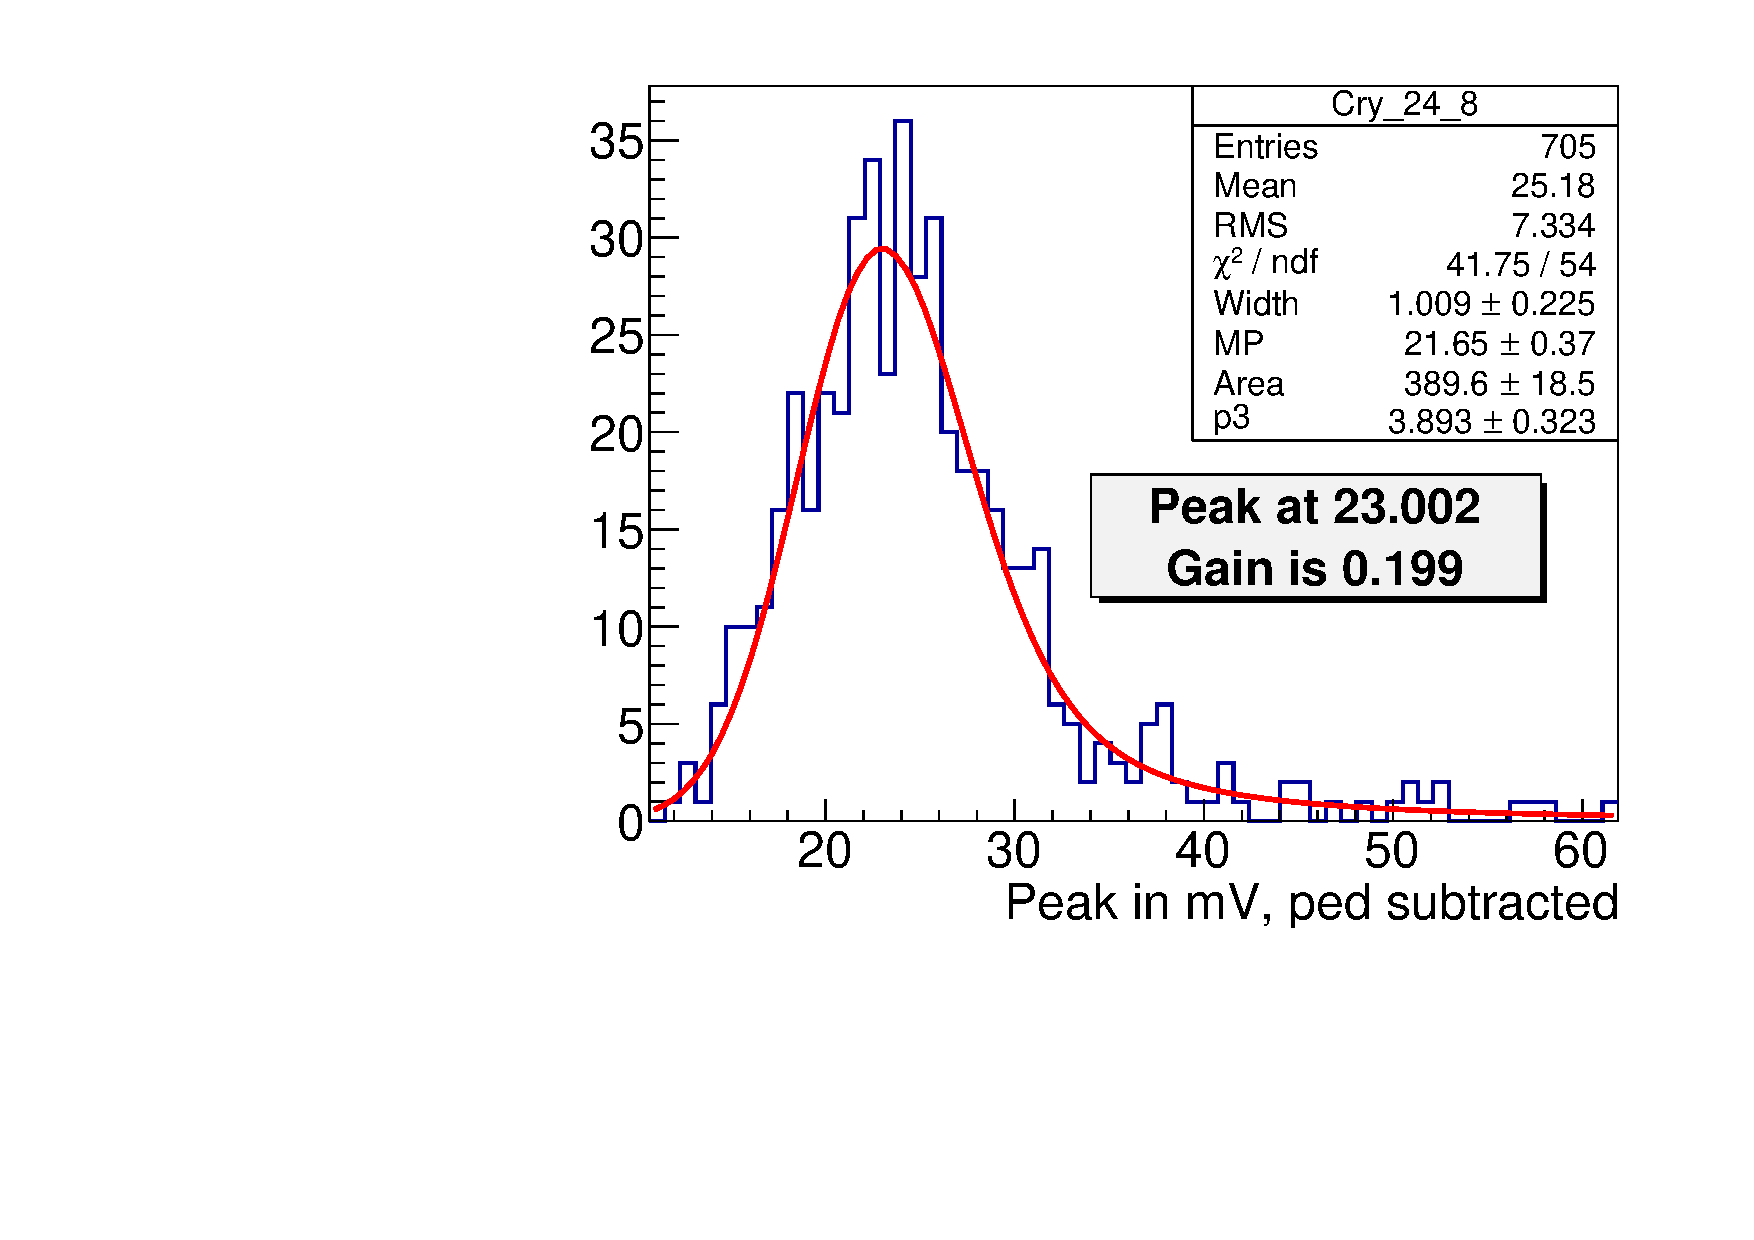
\includegraphics[width=0.8\textwidth]{pics/performance/cosmicFitExample2015.pdf}
  \caption[Integrated cosmic signal in Ecal fitted for calibration]{Each cosmic signal was integrated and then fit using a Landau-Gaussian convolution function. The peak was calculated numerically from this fit.}
  \label{Figure:cosmicFit}
\end{figure}

The fit shown in Fig.~\ref{Figure:cosmicFit} utilized a Landau-Gaussian convolution as the Landau part corresponds to the crystal's response to a particle's energy deposition as ionization energy loss, and the Gaussian part accounts for the statistical nature of the electronics shaping and readout. The peak of the fit is calculated numerically, and the initial conversion from units of FADC to energy (MeV) is obtained (called the Gain factor). The unit conversion from units mV to FADC is 1~V to 4096~FADC. The 4096~FADC counts can be set to 1~V or 2~V, but for 2015 and 2016 running, the setting was 1~V. This arises from the 12~bit conversion which yields 4095~FADC. Using the peak position for crystal in units of FADC, and by knowing the energy deposition of cosmic ray muons from simulation, the gain factor is calculated as shown in Eqn.~\eqref{eq:gain}.

\begin{equation}
	\label{eq:gain}
	Gain = \dfrac{[MeV]}{[FADC]} 
\end{equation}

After approximately 60~hours of cosmic data, the entire Ecal could be calibrated using cosmics, and the resultant gains for all channels in 2015 is shown shown in Fig.~\ref{Figure:cosmicG} and Fig.~\ref{Figure:cosmicGhisto}.

\begin{figure}[H]
  \centering
      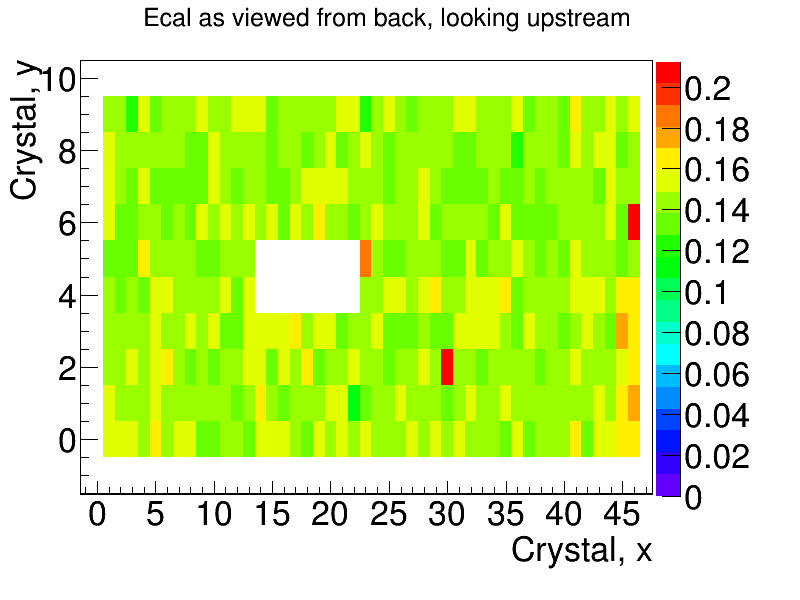
\includegraphics[width=0.7\textwidth]{pics/performance/cosmicGains2015.png}
  \caption[Resulting 2015 gain calibration in the Ecal using cosmic ray muons shown by Ecal module position]{Resulting gain calibration using cosmics for 2015 running (before splitter removal).}
  \label{Figure:cosmicG}
\end{figure}


\begin{figure}[H]
  \centering
      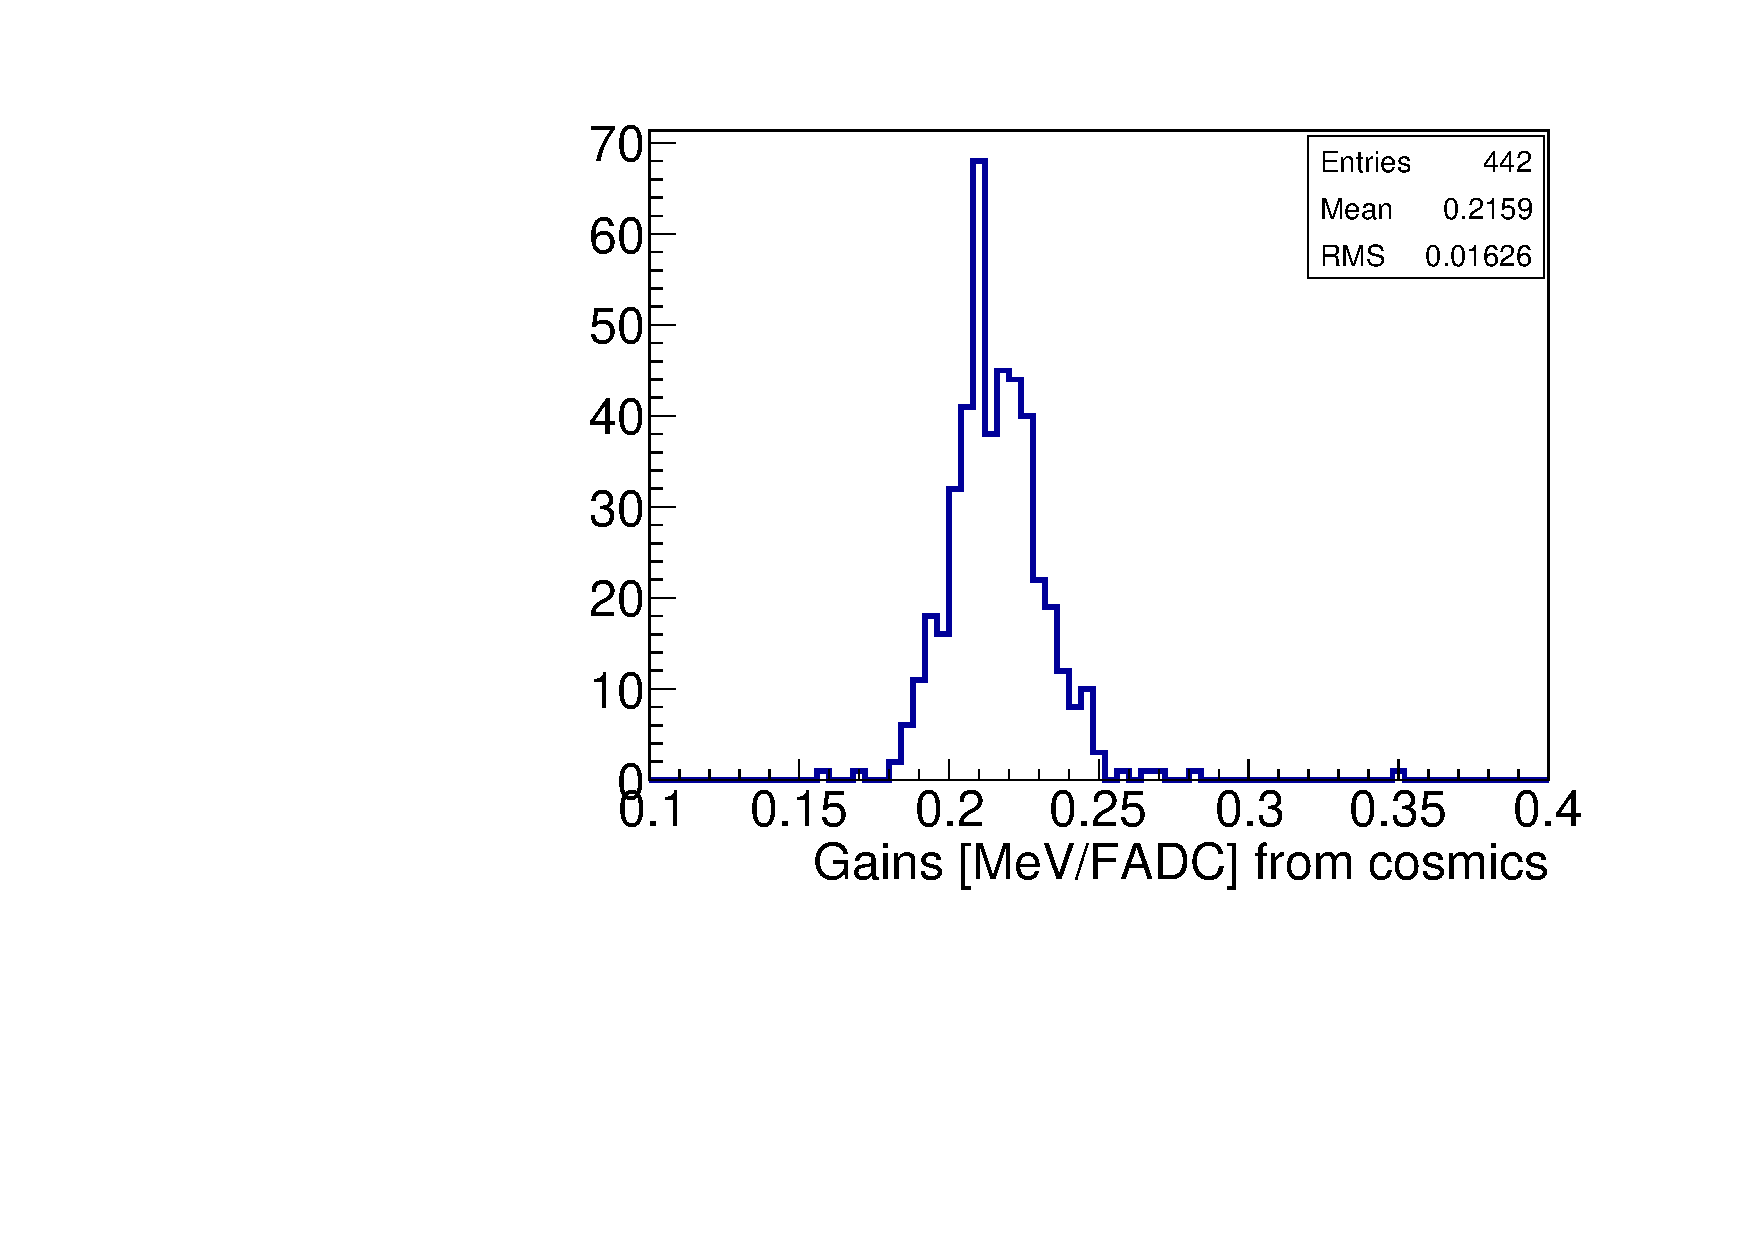
\includegraphics[width=0.7\textwidth]{pics/performance/cosmicGainsMay15.pdf}
  \caption[Distribution of the resulting 2015 gains in the Ecal using cosmic ray muons]{Resulting gain calibration using cosmics for 2015 running (before splitter removal).}
  \label{Figure:cosmicGhisto}
\end{figure}

With the splitters installed the Ecal readout chain, the average gain value was around 0.2~MeV/FADC in 2015. After the removal of the splitters in January 2016, prior to the 2016 Physics Run, the average gains as found by cosmics were around 0.13~MeV/FADC.
